\documentclass[UTF8,fontset=fandol,a4paper,11pt]{ctexart}
\usepackage[left=2.35cm,right=2.35cm,top=2.35cm,bottom=2.35cm]{geometry}
\usepackage{amsmath,amssymb,booktabs,graphicx,float,tabularx,array,enumitem,hyperref,xcolor,tcolorbox}
\tcbuselibrary{breakable}
\hypersetup{hidelinks}
\setlength{\parindent}{2em}
\setlength{\parskip}{0.28em}
\setlength{\emergencystretch}{2em}
\newcommand{\pos}[1]{\left(#1\right)^+}
\newcommand{\keywords}[1]{\par\noindent\textbf{关键词：}#1}
\newtcolorbox{plainbox}[1]{colback=blue!3,colframe=blue!45!black,title=#1,breakable}
\newtcolorbox{limitbox}[1]{colback=orange!4,colframe=orange!65!black,title=#1,breakable}
\title{含光伏与储能微网的风险合同优化与反馈执行详解版\\\large 从信息边界、逐槽平衡到全年策略验证}
\author{}
\date{}

\begin{document}
\maketitle
\thispagestyle{empty}
\begin{abstract}
本版本与正常版使用完全相同的模型、代码、数据和冻结结果，但进一步解释每一层为什么存在。本文把问题概括为“周期预测—残差风险修正—合同层线性规划—真实反馈执行—结算评价”：每天0时只用历史数据、已发布预测和历史误差制定合同；真实负荷与光伏到达当前时槽后，执行器才按光伏、合同、储能、应急的优先级响应。风险备用取历史净负荷残差的0.8分位，这个数来自5倍应急电价的单槽边际权衡。MPC不再承担正式执行，而完整保留为同信息集对照，以检验预测误差环境下不同执行机制的适用性。

典型日需要购电59482.70 kWh，费用35126.95元。2025年2月1日至12月31日334天中，问题二“风险合同LP+反馈执行”总费用1463.69万元，日均4.38万元，应急购电8.06万kWh；在逐日冻结同合同、同初始SOC和同信息的配对实验中，MPC对照费用1642.04万元、应急45.25万kWh，反馈执行节省178.35万元。将预测误差标准差从\(0.5\sigma_0\)放大至\(2.0\sigma_0\)，两者费用差由85.43万元扩大到317.44万元。问题三和问题四相对各自严格同0时信息的冻结合同基线，日内调账分别节省37.56万元和39.99万元。未来扰动不变性、SOC连续性、互斥充放电和母线平衡审计均通过。

\keywords{微网调度；储能；风险合同；线性规划；反馈执行；信息边界}
\end{abstract}

\newpage
\section{先用一句话看懂整道题}

这是一个“明天到底该提前买多少电”的问题。小区白天有光伏、居民要用电，电池可以把暂时多出来的电存起来，也可以在缺电时放出来。真正困难的地方是：决定合同时还不知道明天的真实负荷、光伏和价格；一旦少买，临时补电要付5倍价格；一旦多买，合同电又可能闲置。

四个问题不是四个独立故事，而是一层层把现实困难加进来。微网中的随机建模与优化、模型预测控制和滚动时域方法已有系统研究\cite{liang2014,hu2021,silvente2015}，本文按题目给定的信息时序，把这些思想落实为可核验的预测、合同、执行和结算链条：
\begin{enumerate}[label=第\arabic*步：]
  \item 先假设所有东西都知道，学会安排电池，这是问题一；
  \item 再承认明天的负荷和光伏不知道，必须预测，这是问题二；
  \item 白天拿到新光伏预报，允许改后面的合同，这是问题三；
  \item 最后连未来电价也不知道，需要预测价格，这是问题四。
\end{enumerate}

\begin{plainbox}{先用一句话理解}
整套模型不是把LP、MPC、分位数、CVaR等名词堆在一起，而是让它们各做一件事：预测给出中心值，分位数给出安全余量，LP安排合同与电池，真实反馈处理预测错误，结算公式计算最后花了多少钱。
\end{plainbox}

图\ref{fig:q1-raw}是最直观的起点。负荷高峰、光伏高峰和价格高峰不在同一时间，所以电池有“搬电”的价值。

\begin{figure}[H]
  \centering
  
\includegraphics[width=0.94\textwidth]{figs/raw_q1_typical_profiles.png}
  \caption{典型日的负荷、光伏和电价：三个峰不完全重合}
  \label{fig:q1-raw}
\end{figure}

\section{先把数据单位弄对：kW不是kWh}

每天有144个10分钟时槽。00:10这一行代表00:00--00:10，24:00这一行代表23:50--24:00。附件里的负荷与光伏通常以kW表示，这是功率；电池SOC和购电合同以kWh表示，这是能量。两者不能直接相加。

若某10分钟内功率为\(P_t\) kW，则电量为
\begin{equation}
E_t=P_t\times\frac{10}{60}=\frac{P_t}{6}\quad{\rm kWh}.
\label{eq:conversion}
\end{equation}
例如负荷功率6000 kW持续10分钟，消耗的不是6000 kWh，而是1000 kWh。忘记除以6会把全部能量和费用放大6倍。

全年计算从1月1日开始，但正式费用只统计2月1日至12月31日334天。为什么还要算1月？因为预测需要历史，电池状态也要从前一天连续传到后一天。若每天0时把电池强行恢复6000 kWh，就相当于每天午夜凭空增加或减少电量。

\subsection{原始表格进入模型前做了什么}

第一步是整理时间。附件有的日期只在当天第一行出现，其余行留空，因此先向下填充日期，再给每天的144行编号为\(t=0,1,\ldots,143\)。这里的\(t\)是数组下标，不是钟表上的整点。00:10对应\(t=0\)，00:20对应\(t=1\)，24:00对应\(t=143\)。只有SOC需要145个边界值，因为144段时间有“开始状态”和“结束状态”。

第二步是分开保存“真实值”和“当时能看到的预测值”。真实负荷、真实光伏和真实电价用于模拟事情发生后的结果；官方光伏预报则按发布日期、0/6/12/18时发布时间以及预报提前期单独保存。这样，程序在6时决策时只能读取6时以前发布的版本，不会因为它们恰好放在同一个Excel文件里，就误把下午的真实值当成早上已经知道的信息。

第三步是做最朴素但很重要的检查：日期是否连续、每天是否正好144行、负荷和光伏有没有负值、价格和预报有没有缺失、四个发布时间是否齐全。最后又从程序输出反算一次：合同实际使用量、光伏、放电和应急之和，是否等于负荷和充电之和；SOC是否真的按式\eqref{eq:soc}变化。很多看似“高级模型”的错误，其实来自少一行、错一槽或把kW当kWh，所以这些检查不是附属工作。

\begin{plainbox}{一个时间索引小例子}
假设表中12:10的负荷是6000 kW、光伏是2400 kW。这个槽真实负荷电量是1000 kWh，光伏最多提供400 kWh，尚有600 kWh净需求。若合同提供500 kWh，电池最多放100 kWh就能平衡；若电池不够，缺少部分才记为应急电。程序始终在kWh层面做这个加减。
\end{plainbox}

\section{四条最重要的物理规则}

储能容量是12000 kWh，但只允许使用10%--90%，所以
\begin{equation}
1200\le S_t\le10800.
\label{eq:socbound}
\end{equation}
最大充放电功率为5000 kW，换成10分钟电量就是833.333 kWh。单向效率为0.9，因此电池状态变化为
\begin{equation}
S_{t+1}=S_t+0.9x_t-\frac{y_t}{0.9}.
\label{eq:soc}
\end{equation}

\begin{plainbox}{这条公式表示什么}
\(x_t\)是在交流侧拿去充电的电量。充1 kWh只有0.9 kWh真正留在电池中。\(y_t\)是电池向外送出的电量；要送出1 kWh，SOC要减少\(1/0.9\) kWh。损耗没有消失在数学里，而是写在两个效率系数中。
\end{plainbox}

规划阶段使用预测量：
\begin{equation}
g_t^{\rm P}+v_t^{\rm P}+y_t^{\rm P}=\widetilde L_t+x_t^{\rm P}.
\label{eq:plan}
\end{equation}
真实执行阶段使用真实量：
\begin{equation}
g_t-w_t+v_t^{\rm E}+y_t^{\rm E}+u_t=L_t+x_t^{\rm E}.
\label{eq:execute}
\end{equation}
这里\(g_t\)是已经买下的合同，\(w_t\)是合同中没用掉的部分，\(u_t\)是应急购电。真正从合同进入微网的只有\(g_t-w_t\)，不能把全部合同都假装已经被负荷使用。

为了知道每个字母为什么存在，可以把式\eqref{eq:execute}从右向左读：负荷\(L_t\)和充电\(x_t^{\rm E}\)是这个槽需要电的去向；左边是电从哪里来，包括实际用掉的合同\(g_t-w_t\)、实际用掉的光伏\(v_t^{\rm E}\)、电池放电\(y_t^{\rm E}\)和最后兜底的应急电\(u_t\)。如果光伏太多，用不掉的部分不放进\(v_t^{\rm E}\)，而被记为弃光。每一个变量都对应一种可核对的物理去向。

\begin{plainbox}{为什么必须分“规划”和“执行”}
规划时只能根据预测安排目标SOC；执行时真实负荷和光伏才出现。如果直接把规划SOC当成真实SOC，就等于假装预测永远正确。本文让真实SOC独立递推，预测误差由闲置合同、实际充放电和应急购电共同吸收。
\end{plainbox}

完整的一天可按下面的顺序理解：
\begin{enumerate}[label=第\arabic*步：]
  \item 在决策时刻收集已经可见的信息，生成中心负荷、中心光伏和中心价格预测；
  \item 从过去30个完成日提取误差，形成安全负荷与安全光伏；
  \item 用线性规划求合同和目标SOC曲线；
  \item 真实数据逐槽到达，短时控制器只执行当前动作，随后更新真实SOC；
  \item 新预报到达时只改未来合同，最后按真实价格和真实应急量结算。
\end{enumerate}
这五步的先后顺序比模型名称更重要。只要把第四步提前到第二步，就等于使用未来真实数据；只要每天重新设SOC，就会破坏跨日能量守恒。

\section{问题一：所有数据都知道时，电池怎么搬电}

问题一只需要最小化一天的购电费用：
\begin{equation}
\min C_1=\sum_{t=0}^{143}c_tg_t.
\label{eq:q1objective}
\end{equation}
同时满足电量平衡、SOC边界和功率上限。为了不让模型通过“最后把电池放空”虚假降低当天费用，还要求日末SOC等于日初。

\begin{limitbox}{关于6000 kWh的精确说法}
题面只说0:00和24:00储电量相同，没有额外说这个共同值必须是6000。附件给定2025年1月1日0:00电量为6000 kWh，所以模型先取\(S_0=6000\)，再由循环条件\(S_{144}=S_0\)推出日末也是6000。也就是说，6000来自“给定起点+首尾相等”，不能写成题面另外规定了首尾都必须为6000。
\end{limitbox}

同样最低费用可能对应多条充放电曲线。程序先求最低费用，再在费用不变的解中选择总充放量最小的那条。这样可以排除没有意义的同时充放电。图\ref{fig:q1-process}显示价格与充放电的对应关系，图\ref{fig:q1-result}给出完整轨迹。

为什么这是线性规划？因为目标\(c_tg_t\)对购电量是一次函数，电量平衡和SOC递推都是等式，充放电、光伏利用和SOC上下限也都是线性不等式。因此不需要遗传算法反复碰运气，标准LP求解器能给出全局最优解。第一遍求最低费用后，第二遍把费用限制在最优值的极小容差内，再最小化总充放量。第二遍不是偷偷换目标，而是在同样便宜的方案中选更少折腾电池的一条。

这里还有一个容易误解的地方：充电量20740.662 kWh不是“电池最终多了这么多电”。经过0.9充电效率，真正存进去的是18666.596 kWh；为了向母线放出16799.936 kWh，SOC需要减少约18666.596 kWh。两者正好抵消，所以初末SOC相同。这个手算关系也是对程序结果的独立检查。

\begin{figure}[H]
  \centering
  
\includegraphics[width=0.91\textwidth]{figs/process_q1_price_dispatch.png}
  \caption{问题一：低价时充电、高价时放电的时序关系}
  \label{fig:q1-process}
\end{figure}

\begin{figure}[H]
  \centering
  
\includegraphics[width=0.95\textwidth]{figs/result_q1_optimal_schedule.png}
  \caption{问题一：最优购电、充放电和SOC轨迹}
  \label{fig:q1-result}
\end{figure}

结果为：购电59482.698 kWh，费用35126.949元，充电20740.662 kWh，放电16799.936 kWh，弃光0，SOC范围1200--10800 kWh。平衡误差约\(9.09\times10^{-13}\) kWh，属于浮点计算误差。

\begin{plainbox}{结果为什么可信}
全天首尾SOC相同，所以把状态方程求和后有
\[
  \sum_t y_t=0.81\sum_t x_t.
\]
实际比值为\(16799.936/20740.662\approx0.81\)，正好与两次0.9效率相乘一致。这是一个独立的能量守恒检查。
\end{plainbox}

\section{问题二：明天不知道，合同要怎么买}

\subsection{第一步：做一个只看过去的中心预测}

最终采用F1：明天某时槽的负荷先看7天前同一时槽；光伏看最近7个完成日同槽平均。它简单，但适合数据中的周周期。另有F0和F2作比较，见表\ref{tab:forecast}。

“只看过去”具体意味着：若现在是3月10日0时，要预测3月10日12:10的负荷，F1可以读3月3日12:10的真实负荷，但不能读3月10日早上尚未发生的数据；预测光伏时可以平均3月3日至3月9日12:10的光伏，却不能把3月10日真实天气混进去。等3月10日结束后，它的误差才有资格进入3月11日的残差库。这样的滚动起点评价比随机打乱训练集和测试集更接近真实运营。

MAE是所有绝对误差的平均，回答“典型情况下差多少”；RMSE先平方再平均，对大误差更敏感，回答“有没有少数特别离谱的错误”。净负荷等于负荷减光伏，它直接决定微网需要合同、电池或应急电补上的缺口，所以净负荷误差比单独看负荷误差更接近后续决策。表\ref{tab:forecast}中F1净负荷MAE为273.35 kW，意味着典型10分钟电量误差约为\(273.35/6=45.56\) kWh，但这只是平均尺度，不是每槽固定误差。

\begin{table}[H]
\centering
\caption{预测模型误差比较（kW）}
\label{tab:forecast}
\begin{tabular}{lrrrrrr}
\toprule
模型 & 负荷MAE & 负荷RMSE & 光伏MAE & 光伏RMSE & 净负荷MAE & 净负荷RMSE\\
\midrule
F0 & 722.57 & 904.09 & 335.92 & 557.77 & 804.08 & 1074.83\\
F1 & \textbf{176.80} & \textbf{244.29} & 153.40 & 303.86 & \textbf{273.35} & \textbf{389.97}\\
F2 & 187.90 & 265.74 & 153.40 & 303.86 & 284.35 & 403.25\\
\bottomrule
\end{tabular}
\end{table}

F1误差最小，图\ref{fig:q2-process}也显示大多数预测点靠近真实值。但是，目前只有三者的预测误差比较完成，不能硬说三种预测器都已经跑了完全相同的全年经济闭环，更不能说F1在费用上全面战胜其他模型。

\begin{figure}[H]
  \centering
  
\includegraphics[width=0.88\textwidth]{figs/process_q2_forecast_validation.png}
  \caption{问题二：F1预测与真实观测的比较}
  \label{fig:q2-process}
\end{figure}

\subsection{第二步：把中心预测和风险备用分开}

假设某槽真实净负荷为\(N\)，提前准备\(p\) kWh，普通合同单价为\(c\)，少买部分按\(5c\)补购。暂时忽略储能跨时耦合，单槽损失可写成
\begin{equation}
\ell(p,N)=cp+5c\pos{N-p}.
\label{eq:newsvendor}
\end{equation}
多买1 kWh必付\(c\)，而当\(N>p\)时可避免5倍应急成本。边际平衡满足\(\Pr(N>p)=1/5\)，故风险基准取\(\alpha=0.8\)分位。

\begin{limitbox}{0.8到底表示什么}
它是由价格比导出的单槽经济标尺，不是“全天有80\%概率不缺电”，也不是含144槽联合相关性和储能耦合的概率保证。论文只把它称为风险备用分位，不把它夸大为整日可靠度。
\end{limitbox}

设中心净负荷预测\(\widehat N_t=\widehat L_t-\widehat V_t\)，第\(j\)个完整历史日的净负荷残差为\(e^N_{j,t}=N_{j,t}-\widehat N_{j,t}\)。第\(d\)日0时只允许读取索引区间\([\max(0,d-30),d)\)：今天的真实误差必须等今天结束后，才能进入明天的残差库。将合同分成基础合同\(b_t\)和风险备用\(r_t\)，总合同为\(p_t=b_t+r_t\)。基础部分服务于中心预测：
\begin{align}
b_t+v_t+y_t&=\widehat L_t\Delta t+x_t,\label{eq:risk-base}\\
r_t&\ge\max\{0,Q_{0.8}(e^N_{\cdot,t})\Delta t\}.\label{eq:risk-floor}
\end{align}
再为每个历史日和时槽引入短缺代理\(z_{j,t}\)：
\begin{equation}
z_{j,t}\ge e^N_{j,t}\Delta t-r_t,\qquad z_{j,t}\ge0.
\label{eq:risk-shortfall}
\end{equation}
这相当于询问：“若明天重现某个历史误差，备用之外还会缺多少？”在SOC、功率、光伏利用和能量平衡约束下，合同LP的目标为
\begin{equation}
\min\;\sum_t c_t(b_t+r_t)+5\sum_j\omega_j\sum_t c_tz_{j,t}
-\nu(S_T-S_{\min}).
\label{eq:risk-objective}
\end{equation}
前两项分别是合同费用与历史尾部应急代理；末项是有限时域终端SOC信用，只用于避免规划在日界处无价值地放空，真实结算不会把它当作现金收入。程序把基础合同费、备用合同费和短缺代理分别输出，便于检查目标函数确实按论文实现。

\begin{plainbox}{为什么不把风险备用伪装成预测}
“明天最可能用多少”和“由于少买电很贵，我们额外准备多少”是两个不同问题。F1只回答前者，残差分位和短缺代理回答后者。这样预测精度、风险偏好和合同费用可以分别审计。
\end{plainbox}

\subsection{第三步：真实数据到达后怎样反馈执行}

0时LP输出全天合同，但执行时不照搬其预测充放电轨迹。第\(t\)槽只读取当前真实负荷\(L_t\)、当前真实光伏\(V_t\)、已经买下的合同\(p_t\)和当前SOC，依次执行：
\begin{enumerate}[label=（\arabic*）]
  \item 光伏先供当前负荷；
  \item 合同电补当前剩余负荷；
  \item 若供给有余，余光伏先充电，仍有容量时才吸收余合同；
  \item 若仍有供电缺口，在功率和SOC下限内放电；
  \item 最后无法满足的部分才触发5倍应急购电。
\end{enumerate}
有缺口和有富余是互斥分支，因此不会同槽充放电；应急电只兜底负荷，不允许拿来充电。槽末SOC仍按式\eqref{eq:soc}更新，日末状态直接传给次日。

例如当前负荷1000 kWh、光伏400 kWh、合同500 kWh，则缺口100 kWh由电池放电；若电池已到下限，才应急购电100 kWh。这个动作不需要知道下一槽真实值。所谓反馈，是观察当前状态后纠偏，不是读取未来真实路径。

全年按上述因果闭环回测334天。问题二总费用14636893.76元，日均43823.04元；其中合同费用14142085.22元，应急费用494808.54元。应急购电80648.34 kWh，发生于456个时槽、136个连续事件；闲置合同2037924.81 kWh，弃光1557153.09 kWh。SOC下界为1200 kWh，上界为10800 kWh，年末SOC为10800 kWh。全年反馈执行计算时间为0.169秒。全年净负荷结构与连续SOC轨迹分别见图\ref{fig:q2-raw}和图\ref{fig:q2-soc}。

\begin{figure}[H]
  \centering
  
\includegraphics[width=0.96\textwidth]{figs/raw_q2_annual_netload.png}
  \caption{问题二：全年净负荷的季节与日内结构}
  \label{fig:q2-raw}
\end{figure}

\begin{figure}[H]
  \centering
  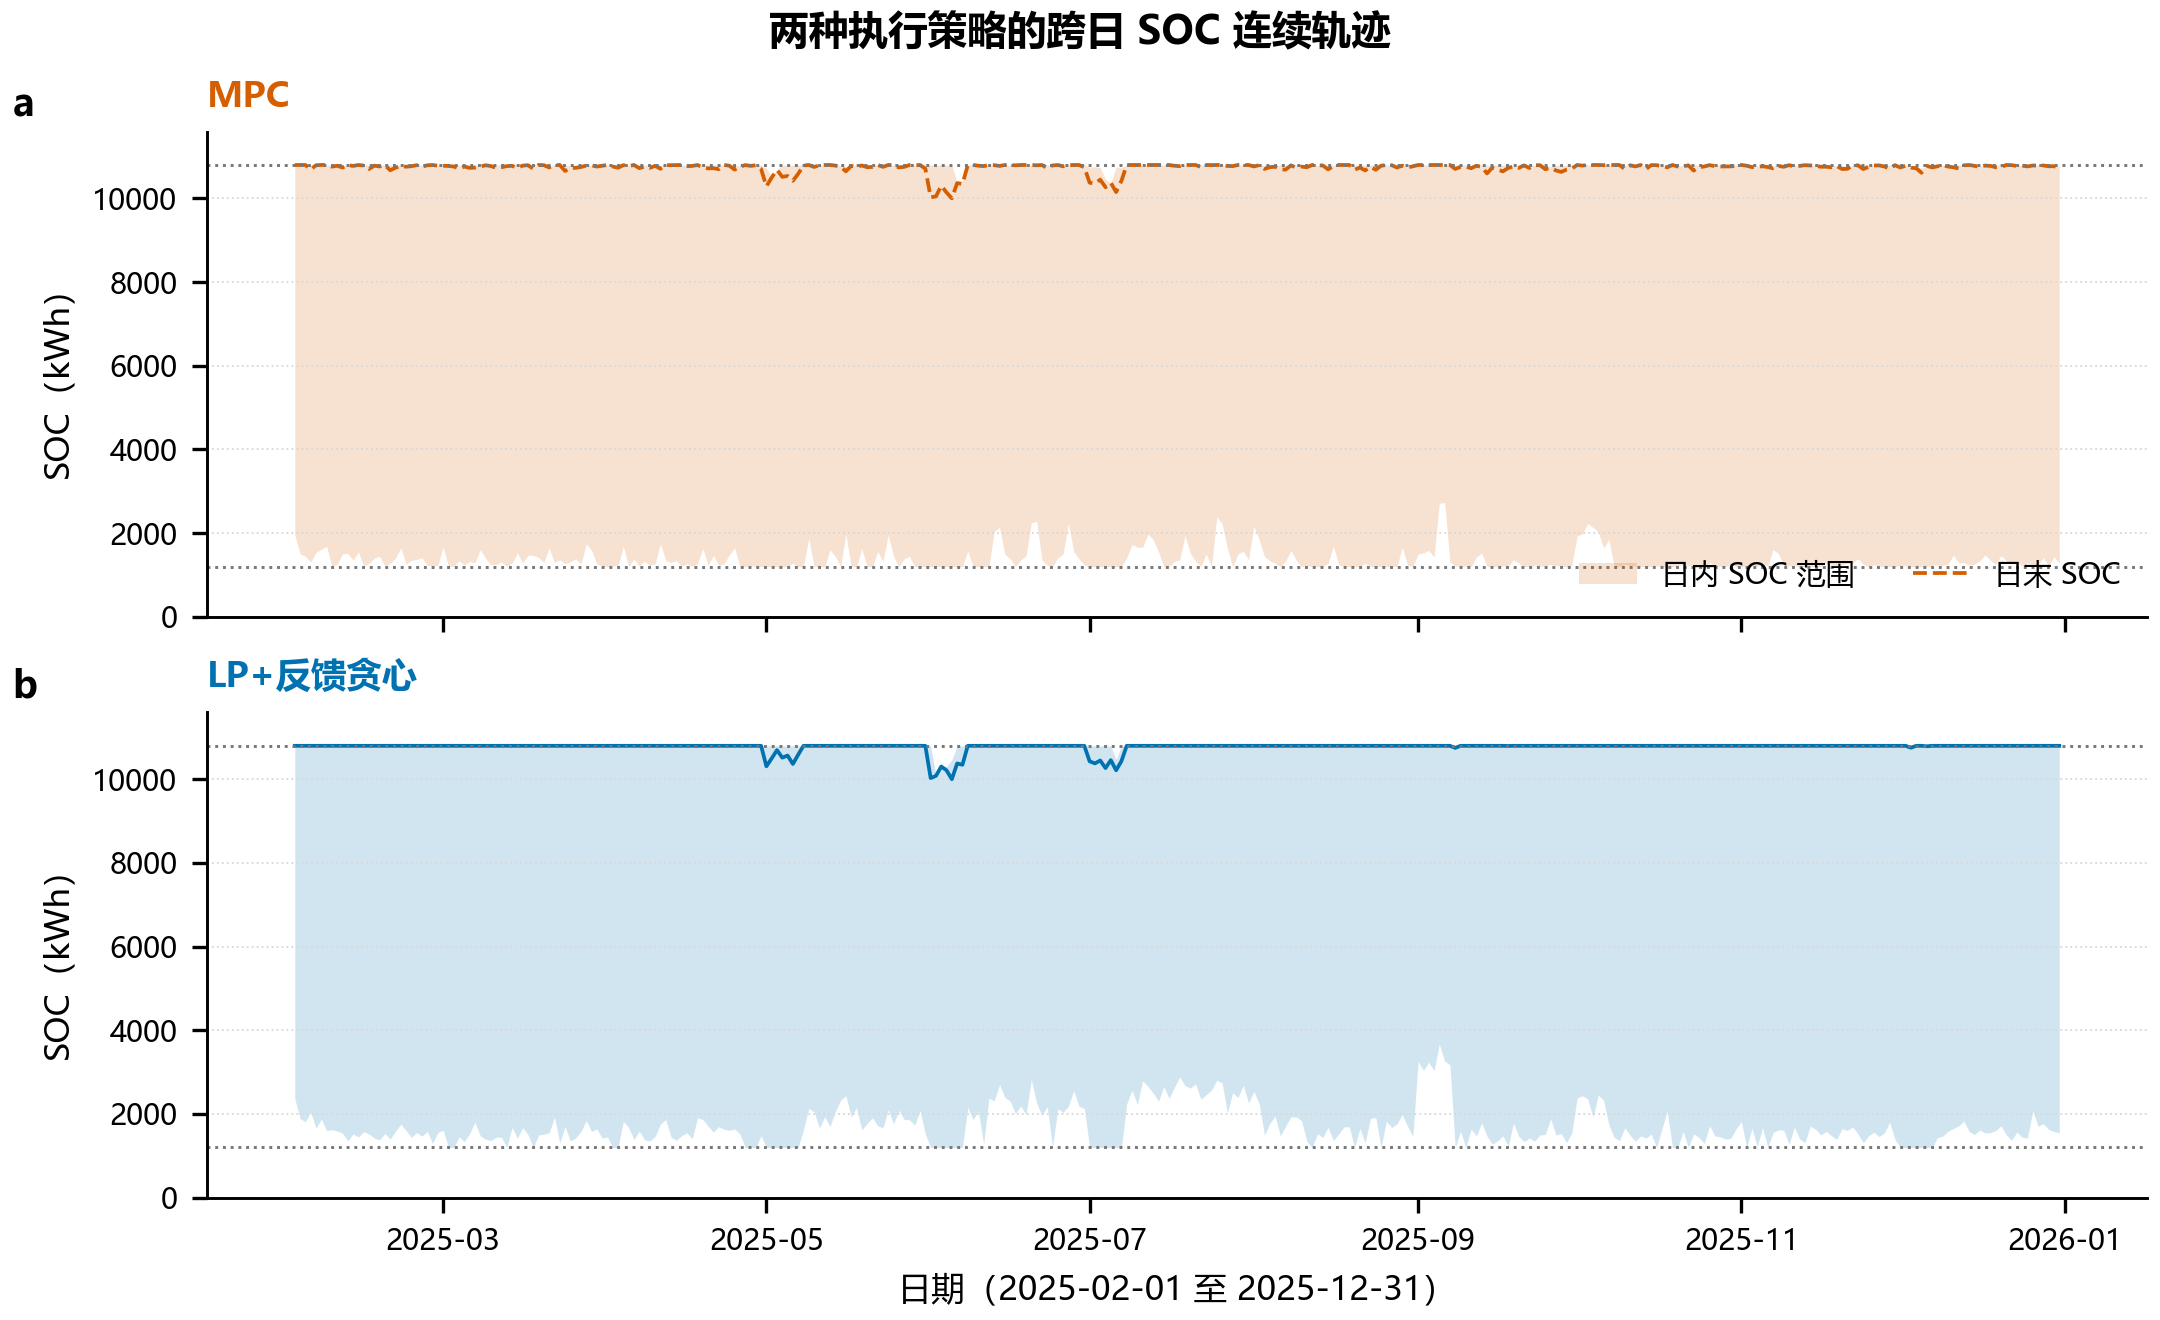
\includegraphics[width=0.95\textwidth]{figs/q2_soc_continuity.png}
  \caption{问题二：两种执行策略的全年SOC连续轨迹}
  \label{fig:q2-soc}
\end{figure}

\begin{plainbox}{为什么年末10800 kWh不违反题意}
问题二没有要求每天午夜或年末回到6000 kWh。程序既没有每天重置SOC，也没有凭空补电；10800 kWh只是连续执行334天后的合法终点，并且未超过90\%容量上限。
\end{plainbox}

\section{问题三：新预报到达后，只调整未来合同}

\subsection{调账LP与真实反馈各做什么}

0、6、12、18时发布的官方光伏预报先映射到10分钟网格，再用相同发布时间和提前期的历史误差修正。每次更新都从真实当前SOC开始，只重算尚未执行的合同；已发生的能量流、费用和SOC前缀永久冻结。执行层依然采用问题二的当前槽反馈规则，日内LP只负责改变合同，不接管真实充放电。合同更新的因果时序见图\ref{fig:q3-process}。

\begin{figure}[H]
  \centering
  
\includegraphics[width=0.95\textwidth]{figs/process_q3_contract_updates.png}
  \caption{问题三：每次新信息只改变尚未执行的合同}
  \label{fig:q3-process}
\end{figure}

设0时基准合同为\(p_t\)，调账后生效合同为\(q_t\)，应急电为\(u_t\)。主结算采用
\begin{equation}
C_t=c_t[\min(p_t,q_t)+1.5\pos{q_t-p_t}+0.5\pos{p_t-q_t}]+5c_tu_t.
\label{eq:settlement}
\end{equation}
例如原合同10 kWh、下调到5 kWh、单价1元，则保留5 kWh付5元，取消5 kWh付2.5元，共7.5元；若原合同5 kWh、上调到10 kWh，则共付12.5元。另一种“原合同全付再另加下调罚金”的字面解释，会使下调越多反而越贵，因此只作为替代结算对同一物理轨迹重计费，不在替代规则下重新优化。

对未执行时槽引入上、下调量\(\delta_t^+,\delta_t^-\ge0\)，更新后的基础合同与备用满足
\begin{equation}
b_t+r_t=p_t+\delta_t^+-\delta_t^-.
\label{eq:adjust-relation}
\end{equation}
更新LP保留式\eqref{eq:risk-base}--\eqref{eq:risk-shortfall}的风险约束，并将目标改为
\begin{equation}
\min\;\sum_t c_t(p_t+1.5\delta_t^+-0.5\delta_t^-)
+5\sum_j\omega_j\sum_t c_tz_{j,t}-\nu(S_T-S_{\min}).
\label{eq:adjust-objective}
\end{equation}
同槽同时增加等量上调和下调会严格增加目标，因此最优解不会借此制造虚假交易。代码还使用次级吞吐优化，在相同主目标下排除没有物理意义的多余充放电。

\subsection{为什么必须设置严格冻结基线}

问题三主费用14426279.48元，替代结算费用15118551.31元；应急32292.76 kWh，闲置1579427.50 kWh，弃光1384142.51 kWh。0时初始合同总量22973737.44 kWh，日内最终生效合同22141520.73 kWh。

若直接拿问题二比较，0时光伏预测来源也发生了变化，因此两者210614.28元差额只能称为“完整策略差异”。为识别调账本身的效果，程序新增\texttt{q3\_no\_adjust}：它与问题三共享0时官方预报、F1负荷预测、30日残差、风险LP、初始SOC和反馈执行器，唯一差别是关闭6、12、18时调账。该严格基线费用14801900.59元，应急80831.62 kWh，闲置2314004.19 kWh，弃光1540373.23 kWh。

因此，日内调账的纯净效应是节省375621.11元，即2.54\%；应急、闲置和弃光分别减少48538.86、734576.69和156230.72 kWh。图\ref{fig:q3-result}画的是这一组严格配对，而不是把信息集不同的两条主线硬作因果比较。

\begin{figure}[H]
  \centering
  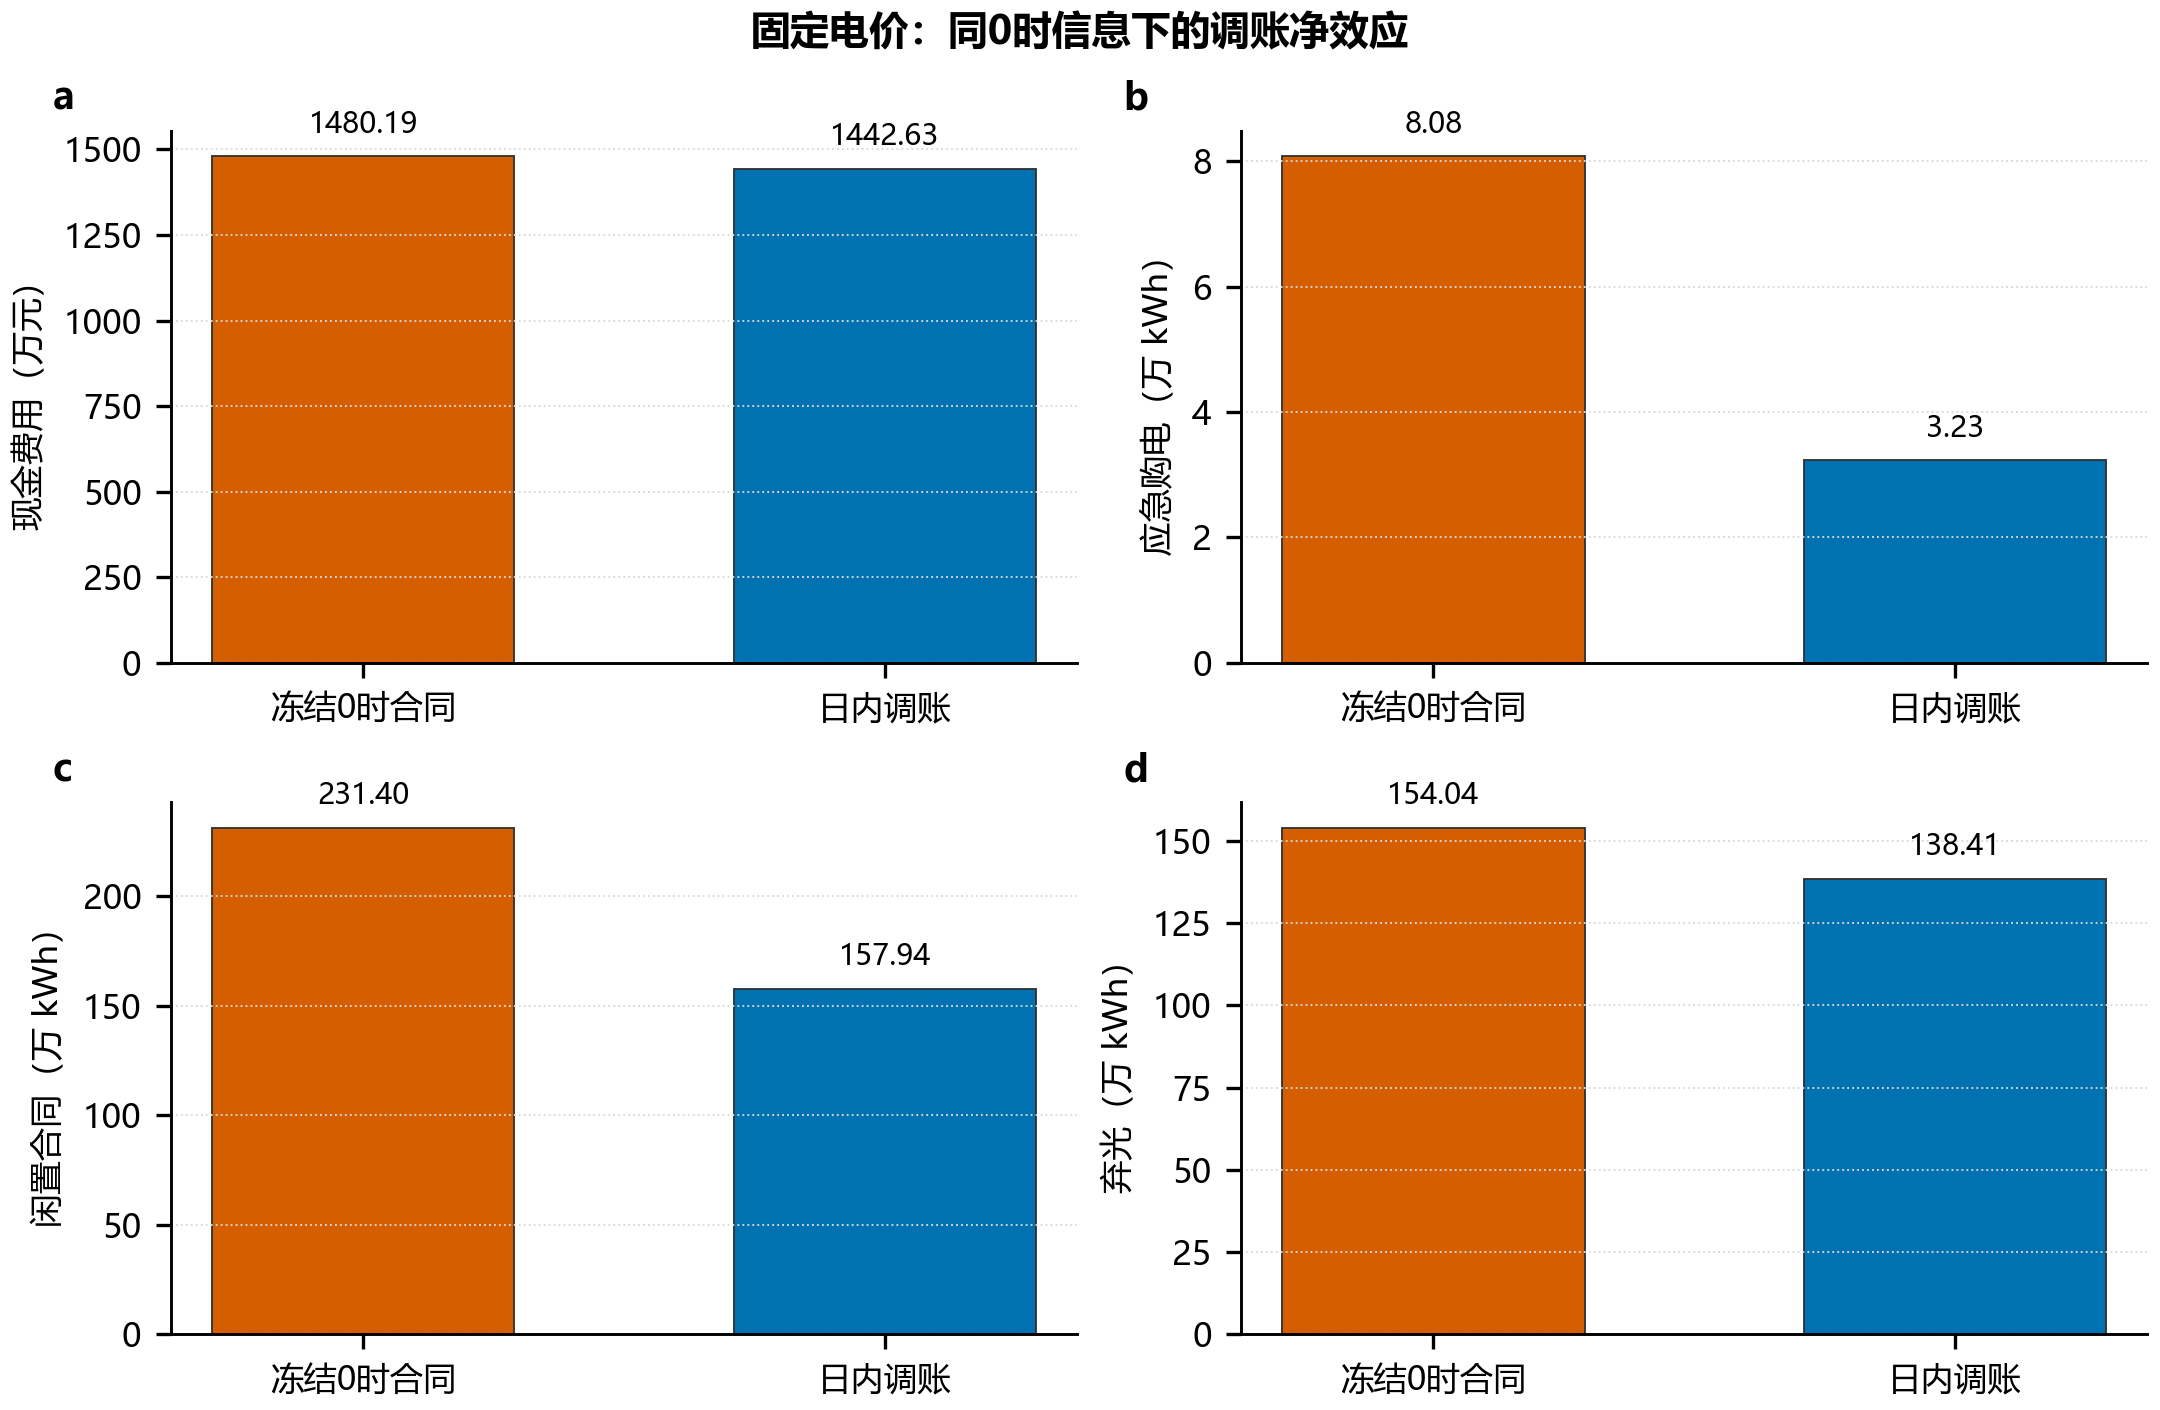
\includegraphics[width=0.93\textwidth]{figs/q3_greedy_adjustment_comparison.png}
  \caption{固定价下同0时信息的冻结合同与日内调账比较}
  \label{fig:q3-result}
\end{figure}

\section{问题四：变动电价也必须遵守信息时序}

问题四给出了事后真实价格，但0时决策不能直接读取当天未来价。本文以过去30个完成日同槽价格中位数作为0时预测，日内仅用已经实现的价格偏差作指数衰减修正；真实未来价格只负责最终现金结算。真实价格波动见图\ref{fig:q4-raw}，预测价、结算价与储能动作的关系见图\ref{fig:q4-process}。

\begin{plainbox}{预测价和结算价不是一回事}
预测价回答“此刻应给未来留多少电”，真实价回答“事情发生后实际付了多少”。把全天真实价提前放进目标函数会形成完美信息优势，得到无法实施的理想结果。
\end{plainbox}

\begin{figure}[H]
  \centering
  
\includegraphics[width=0.91\textwidth]{figs/raw_q4_price_variability.png}
  \caption{问题四：真实价格的日期—时刻波动}
  \label{fig:q4-raw}
\end{figure}

\begin{figure}[H]
  \centering
  
\includegraphics[width=0.92\textwidth]{figs/process_q4_price_dispatch.png}
  \caption{问题四：预测价格、结算价格与储能调度}
  \label{fig:q4-process}
\end{figure}

反馈执行下，无调账题面分支费用15323615.30元，应急78919.00 kWh，闲置2006526.78 kWh，弃光1590815.54 kWh；有调账分支主费用15123873.94元，替代结算费用15837670.08元，应急31843.63 kWh，闲置1532390.95 kWh，弃光1413872.53 kWh。二者完整策略差为199741.36元，但0时光伏预测来源不同，不能称为纯调账收益。

严格基线\texttt{q4\_3\_no\_adjust}与有调账分支共享全部0时信息、价格预测、残差、SOC和执行器，仅关闭日内调账。其费用15523743.57元，应急80088.17 kWh，闲置2279304.66 kWh，弃光1577024.02 kWh。因此调账净节省399869.63元，即2.58\%；应急、闲置和弃光分别减少48244.53、746913.72和163151.49 kWh。严格配对结果见图\ref{fig:q4-result}。

\begin{figure}[H]
  \centering
  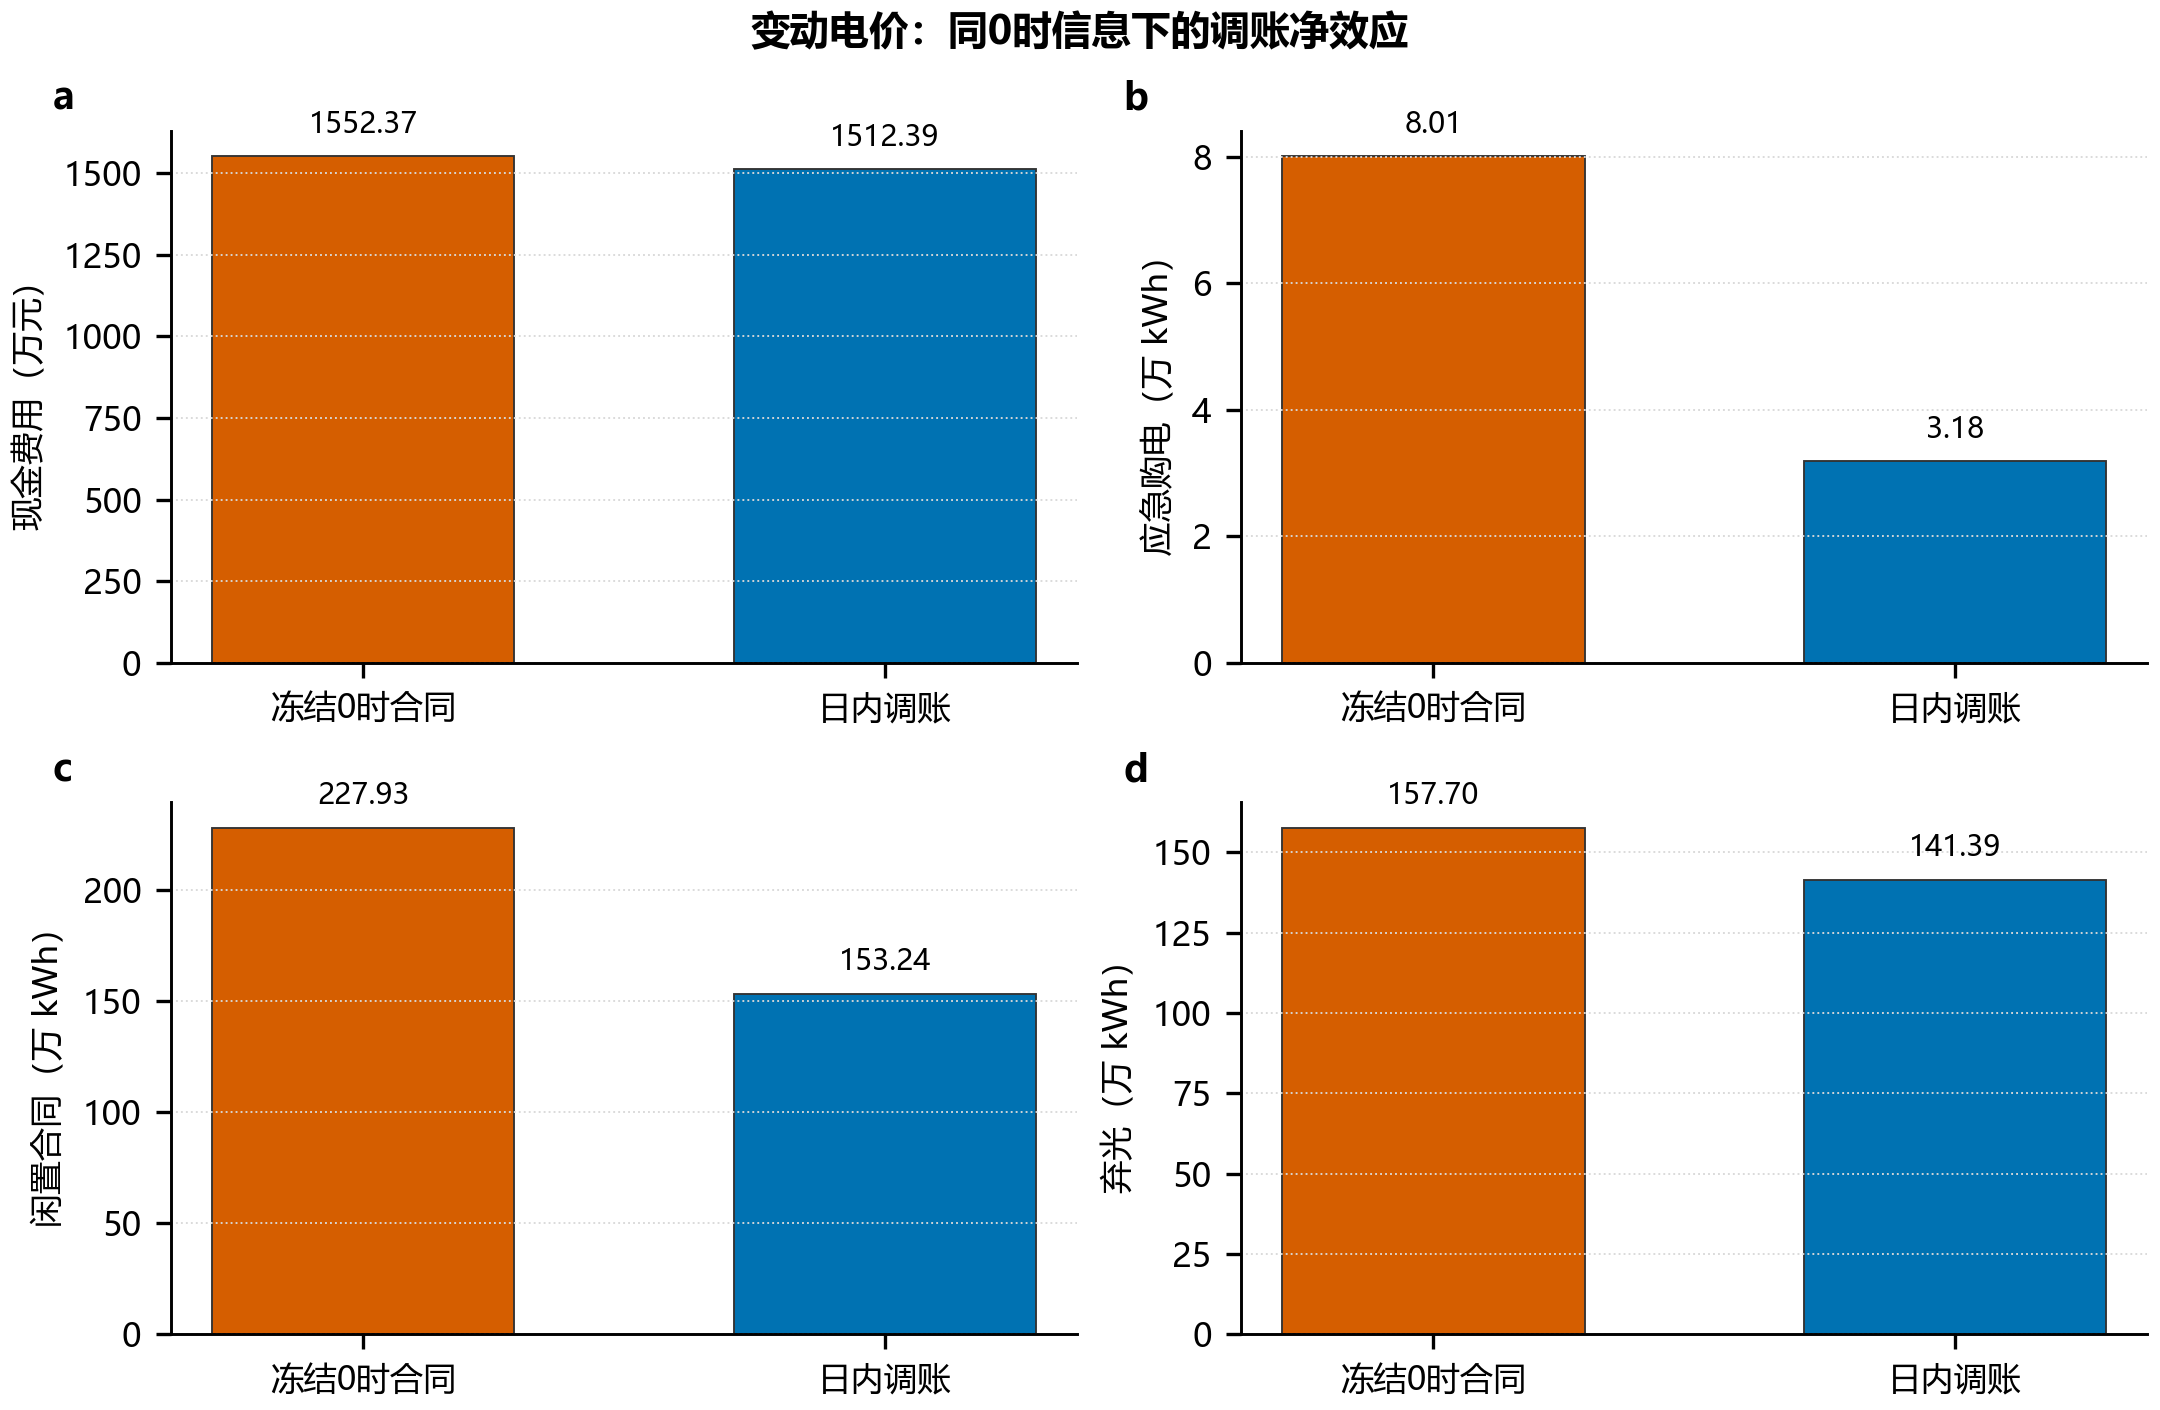
\includegraphics[width=0.92\textwidth]{figs/q4_greedy_adjustment_comparison.png}
  \caption{变动电价下同0时信息的冻结合同与日内调账比较}
  \label{fig:q4-result}
\end{figure}

四个题面主分支的年度现金费用和能量指标汇总见表\ref{tab:main}。

\begin{table}[H]
\centering
\caption{四个题面主分支的334日结果}
\label{tab:main}
\resizebox{\textwidth}{!}{%
\begin{tabular}{lrrrr}
\toprule
策略 & 现金费用/元 & 应急/kWh & 闲置合同/kWh & 弃光/kWh\\
\midrule
问题二：固定价、0时合同 & 14636893.76 & 80648.34 & 2037924.81 & 1557153.09\\
问题三：固定价、日内调账 & 14426279.48 & 32292.76 & 1579427.50 & 1384142.51\\
问题四--2：变价、0时合同 & 15323615.30 & 78919.00 & 2006526.78 & 1590815.54\\
问题四--3：变价、日内调账 & 15123873.94 & 31843.63 & 1532390.95 & 1413872.53\\
\bottomrule
\end{tabular}}
\end{table}

\section{执行策略选择与验证}

\subsection{MPC作为同信息集对照，而不是正式执行层}

保留的\texttt{baseline\_MPC()}只作执行器对照。配对实验逐日冻结反馈主线已生成的日前合同和日初SOC，并向两种执行器提供完全相同的预测路径、真实路径与结算价。差别只在当前动作：MPC每槽根据可见预测求有限时域LP并执行第一步；反馈策略只读当前真实供需和SOC，按固定优先级执行。全年冻结同输入配对见表\ref{tab:controller}和图\ref{fig:q2-controller}；各自连续跨日闭环另作辅助诊断，不与这里的因果对照口径混用。

\begin{table}[H]
\centering
\caption{相同信息集下的334日执行策略比较}
\label{tab:controller}
\begin{tabular}{lrrrr}
\toprule
执行策略 & 总费用/元 & 应急/kWh & 闲置合同/kWh & 计算时间/s\\
\midrule
MPC对照 & 16420412.62 & 452547.46 & 2267443.46 & 375.186\\
LP+反馈执行 & 14636893.76 & 80648.34 & 2037924.81 & 0.156\\
\bottomrule
\end{tabular}
\end{table}

反馈执行减少费用1783518.86元，降幅10.86\%，应急减少371899.12 kWh，执行计算约快2410倍。这里的结论是“不同执行策略在本题误差结构下适用性不同”，不是“MPC失败”。MPC能显式表达未来视野和目标SOC，但预测偏差与有限时域末端价值会影响当前动作；反馈策略直接处理已经发生的供需缺口，在5倍应急价格下更稳健。

\begin{figure}[H]
  \centering
  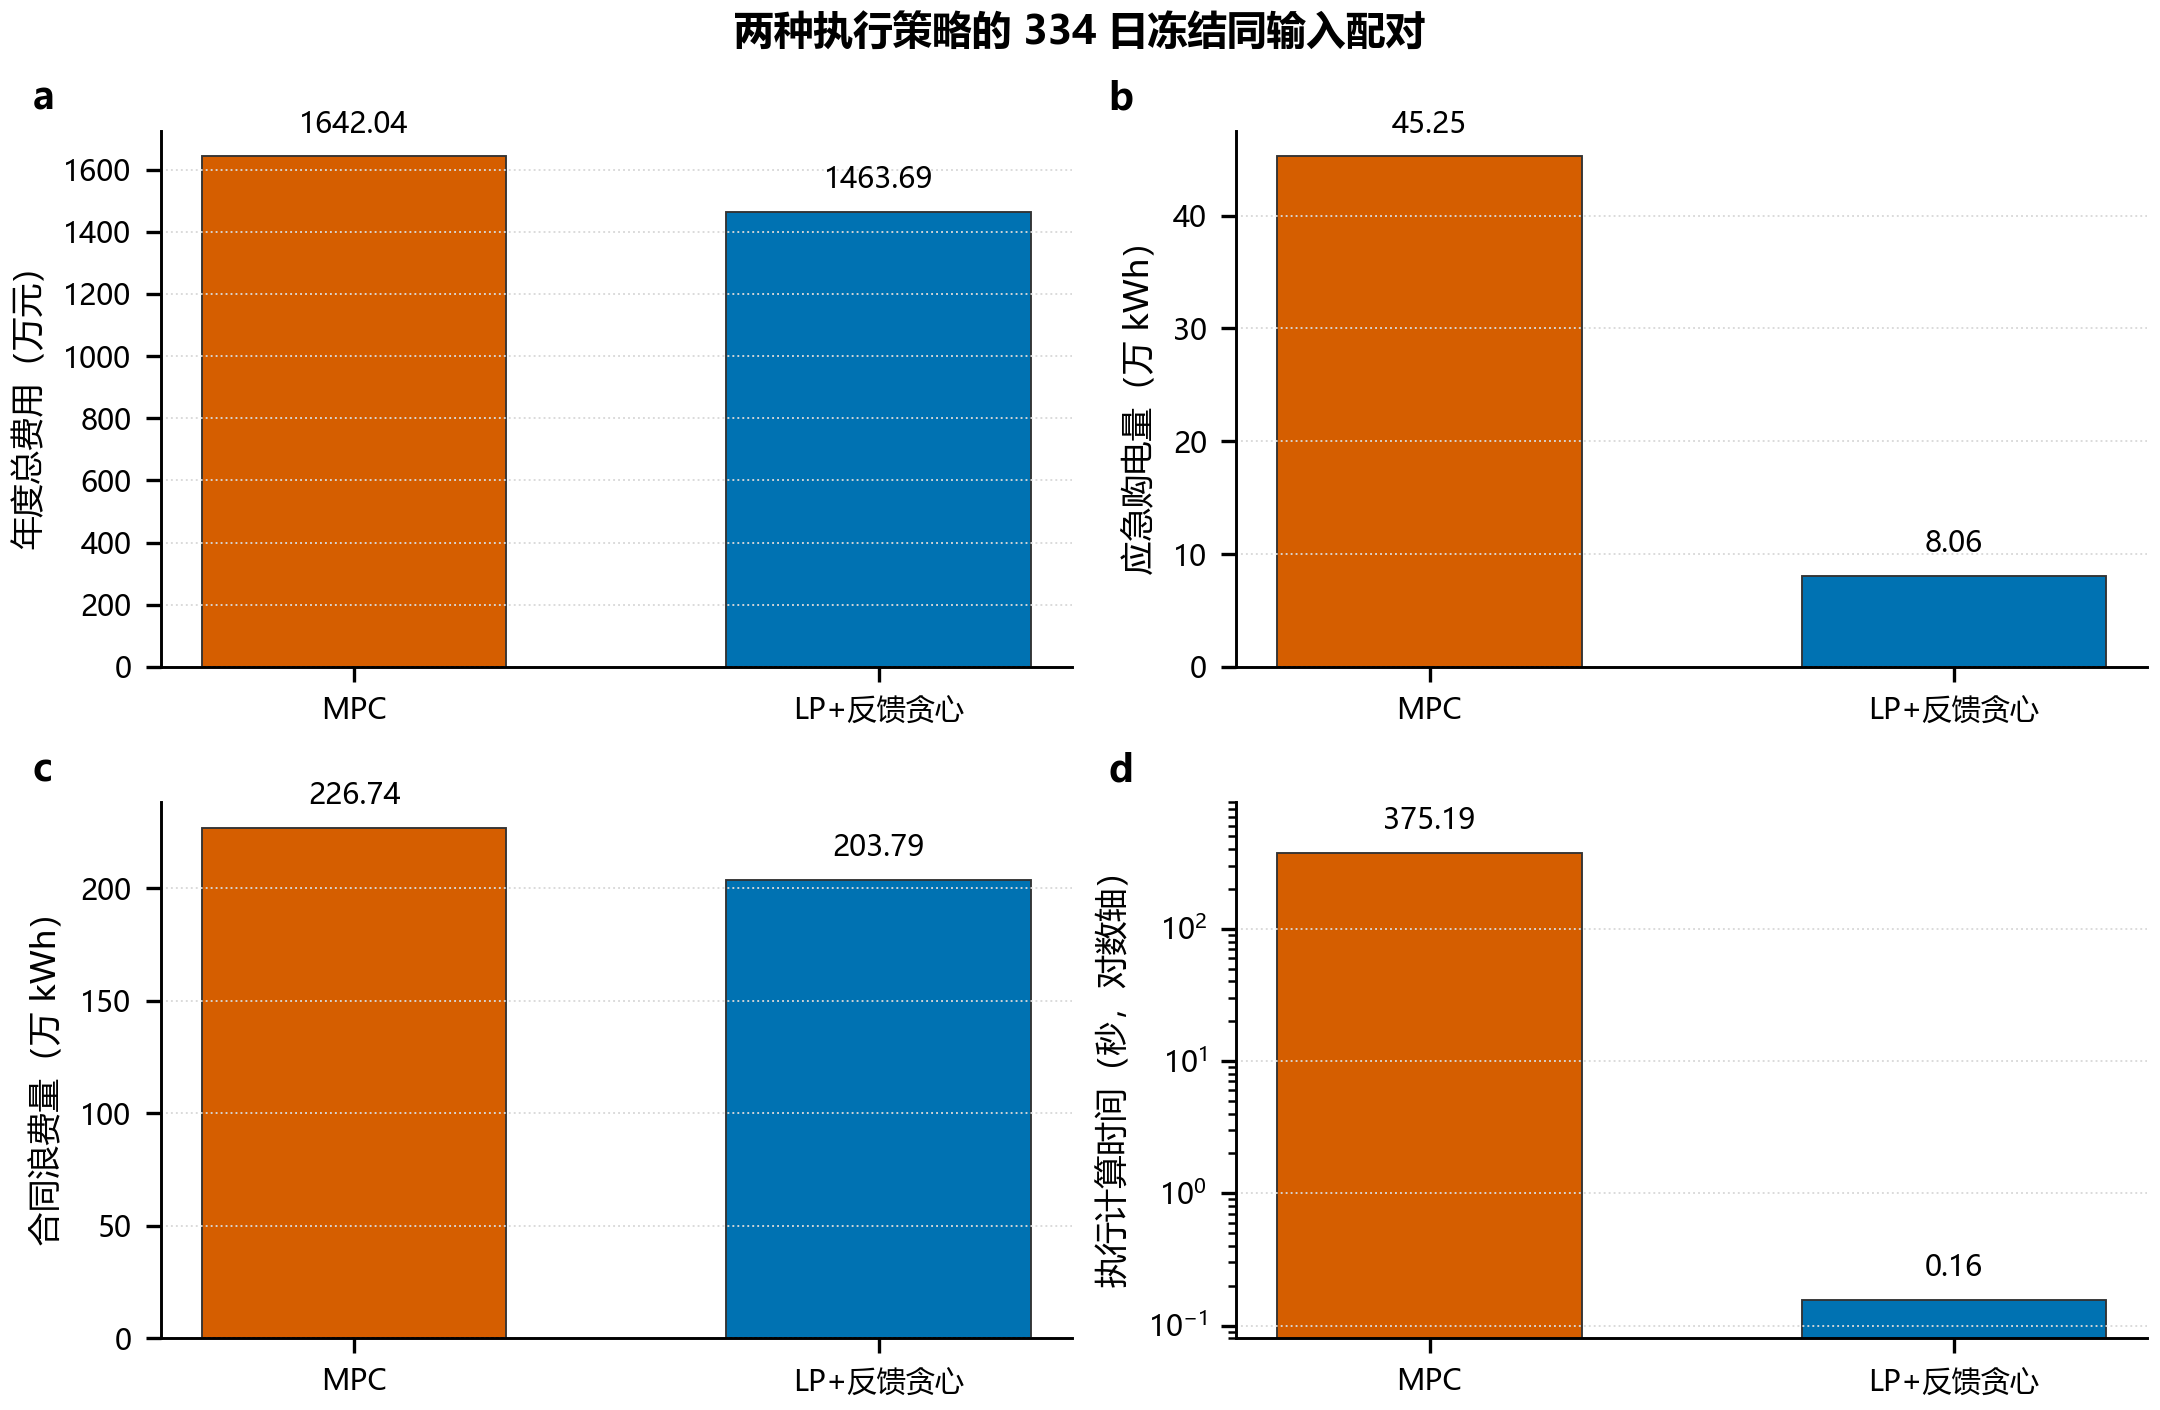
\includegraphics[width=0.95\textwidth]{figs/q2_execution_strategy_comparison.png}
  \caption{两种执行策略的334日冻结同输入配对}
  \label{fig:q2-controller}
\end{figure}

\subsection{预测误差放大后会怎样}

固定日前合同和两种方法的信息集，只把真实净负荷残差标准差调为\(0.5,1.0,1.5,2.0\)倍基准。MPC减反馈执行的年度费用差依次为854285.52、1783518.86、2543268.41和3174376.67元。随着误差增加，MPC应急量由16.73万kWh增至116.33万kWh，反馈策略由0.38万kWh增至41.77万kWh；两者都受误差影响，但反馈策略增长更慢，具体趋势见图\ref{fig:q2-error}。

\begin{figure}[H]
  \centering
  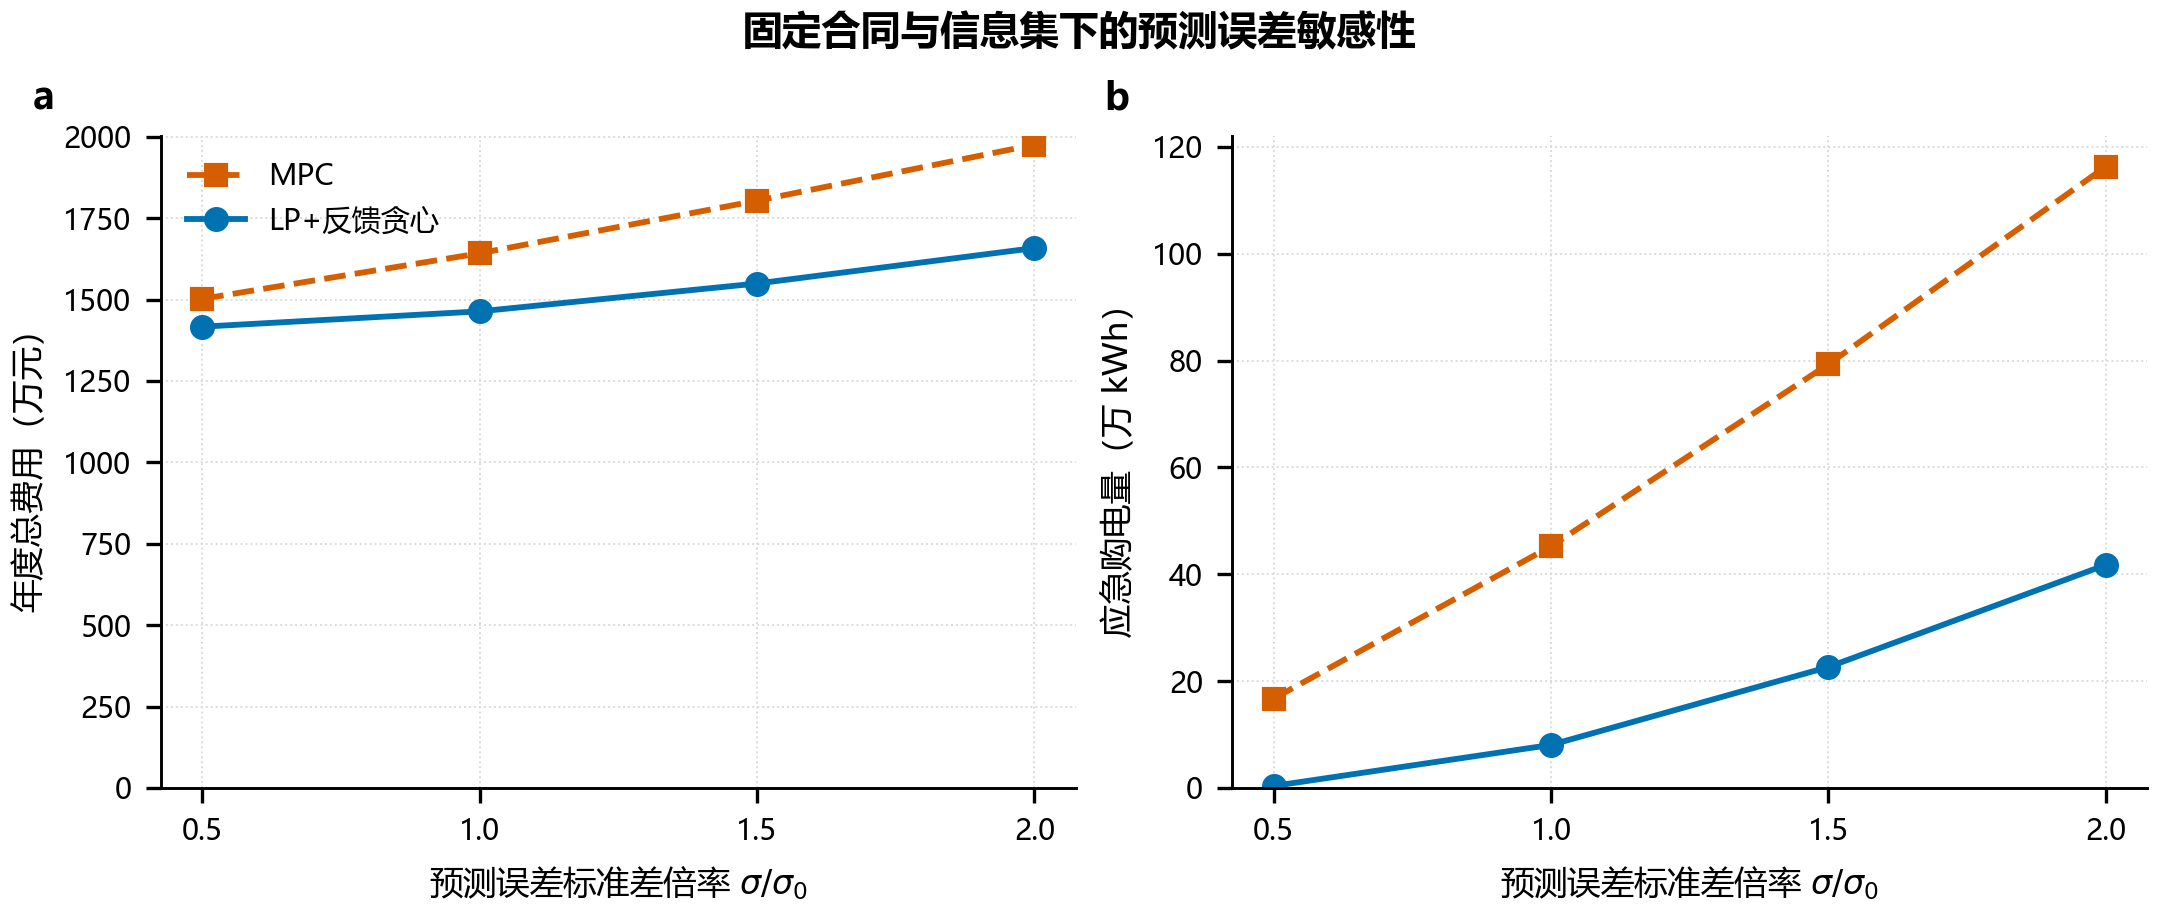
\includegraphics[width=0.95\textwidth]{figs/q2_error_sensitivity.png}
  \caption{相同合同与信息集下的预测误差敏感性}
  \label{fig:q2-error}
\end{figure}

\begin{plainbox}{敏感性实验能证明到哪一步}
它支持“在本数据、当前电池参数和5倍应急价下，误差越大，反馈执行相对更稳定”。它没有证明反馈在所有电价、电池容量或预测模型下都必然优于MPC。
\end{plainbox}

\subsection{信息公平性：知道当前不等于偷看未来}

在2025年3月20日的扰动实验中，合同残差历史窗口固定为\([48,78)\)，把第48槽及之后的真实负荷与光伏换成另一条路径。日前合同最大差异为0；反馈与MPC在前48槽的动作最大差异均为0，SOC最大差异也为0。若程序偷看了未来，修改未来数据就会反过来改变早先动作；测试没有出现这种现象。

这个实验保证两种执行器面对同一可见信息。反馈执行在当前槽读取当前真实值，是实际运行必须有的测量；MPC也在相同时刻取得相同当前状态。未来预测可以使用，但未来真实负荷、真实光伏和真实价格均不可使用。

\section{程序、模型和结果怎样互相核对}

代码层共有15项核心测试通过，结果评价测试与年度风险合同审计也通过。正式问题二回测的最大母线平衡残差为\(2.27\times10^{-13}\) kWh；SOC范围1200--10800 kWh；同时充放电槽数为0；应急电充电槽数为0。问题三、四的逐槽CSV还与年度汇总交叉核对，日期完整覆盖334天，日末SOC等于次日日初SOC。

\begin{plainbox}{“求解成功”为什么还不够}
求解器返回最优只说明它忠实解了输入方程。可信结果还要通过四层检查：原始时间轴与单位、方程回代与SOC连续、未来扰动不变性、论文数字与CSV/工作簿交叉核对。四层分别防止数据错、数学错、信息泄露和写作夸大。
\end{plainbox}

风险合同LP的目标分解也被单独检查：合同项、备用项、历史短缺代理和终端信用之和与求解器目标在容差内一致；调账LP满足式\eqref{eq:adjust-relation}，且同槽上、下调不并存。这样，论文写出的“风险合同”和“调账”确实对应代码变量，而不是事后给旧程序换名字。

\section{三项创新与模型边界}

\begin{enumerate}[label=（\arabic*）]
  \item \textbf{预测误差驱动的安全轨迹合同优化。} 中心预测形成基础合同，0.8分位形成最低风险备用，历史尾部短缺代理进入LP目标；三部分都能从输出中单独追溯。
  \item \textbf{合同决策与真实执行解耦。} 日前LP严格停留在0时信息集，真实执行只读取当前槽观测；合同可以提前优化，预测错误则由状态反馈吸收。
  \item \textbf{预测控制与反馈控制的适用性比较。} MPC保留为逐日冻结同合同、同初始SOC和同信息的全年配对对照，并通过误差敏感性与未来扰动实验补足“为什么选反馈”的证据链。
\end{enumerate}

模型优势是线性、透明、全年可复现，而且把预测、风险、交易、执行和结算的职责分开。局限也要明确：逐槽分位和历史短缺代理不能给出整日联合机会约束；F1依赖周周期，节假日或结构突变时可能失效；反馈优先级没有显式计入电池老化，也不保证事后全局最优；配电网潮流、需求响应和售电机制尚未建模。当前MPC对照只说明本样本与参数下的适用性，不能外推成控制理论上的普适排序。

\begin{limitbox}{本文不能宣传的结论}
不能写成“完整随机MPC”“整日80\%可靠度”“反馈策略普适最优”或“MPC失败”。准确说法是：根据本题的信息结构、实测预测误差和5倍应急价格，风险合同LP配合当前槽反馈在全年同信息集对照中表现更稳定。
\end{limitbox}

\section{最终结论与实施建议}

问题一典型日费用35126.95元，并澄清6000 kWh来自给定初态和首尾相等。问题二在F1、0.8风险备用、风险合同LP和反馈执行下，总费用1463.69万元，应急8.06万kWh；相对冻结同合同、同日初SOC和同信息的MPC配对对照节省178.35万元，应急减少37.19万kWh。误差放大时两者费用差持续扩大，支持选择反馈执行作为本题正式策略。

问题三日内调账费用1442.63万元，相对严格冻结基线净节省37.56万元；问题四变价日内调账费用1512.39万元，相对其严格基线净节省39.99万元。只有这两组冻结基线差额才被解释为调账净效应，问题二与三、问题四两个题面分支之间的差额只作完整策略描述。

实际部署可分两步：先影子运行“0时风险合同+当前槽反馈”，每日核对合同、SOC、应急和结算；数据接口稳定后，再在6、12、18时开放题目允许的合同调账。迁移到其他年份时，应重新校准30日残差窗口、风险分位和终端SOC价值；若应急倍率、电池容量或误差结构改变，也应重新运行反馈与MPC的公平对照。

\section*{AI工具使用声明}

本详解版在资料整理、代码审查、结果核对、LaTeX排版和语言解释阶段使用了人工智能辅助工具。模型、假设、数字和结论仍须由参赛队伍结合原题与附件逐项理解、核验和改写，并承担最终学术责任。本稿是学习和人工复核材料，不应未经审查直接提交。

\begingroup
\raggedright
\begin{thebibliography}{9}
\bibitem{liang2014} Liang H., Zhuang W. Stochastic Modeling and Optimization in a Microgrid: A Survey. \emph{Energies}, 2014, 7(4): 2027--2050. DOI: 10.3390/en7042027.
\bibitem{hu2021} Hu J., Shan Y., Guerrero J. M., et al. Model Predictive Control of Microgrids---An Overview. \emph{Renewable and Sustainable Energy Reviews}, 2021, 136: 110422. DOI: 10.1016/j.rser.2020.110422.
\bibitem{silvente2015} Silvente J., Kopanos G. M., Pistikopoulos E. N., Espu\~na A. A Rolling Horizon Stochastic Programming Framework for the Energy Supply and Demand Management in Microgrids. \emph{Computer Aided Chemical Engineering}, 2015, 37: 2057--2062. DOI: 10.1016/B978-0-444-63576-1.50081-9.
\end{thebibliography}
\endgroup

\newpage
\appendix
\section{怎样复现主结果}

冻结配置是随机种子2026、F1预测、30日未聚类净负荷残差、\(\alpha=0.8\)和\texttt{greedy}反馈执行。正式执行不含MPC视野或SOC跟踪权重；36槽参数只属于\texttt{baseline\_MPC()}对照。在项目根目录运行：
\begin{verbatim}
python -X utf8 run_q2_strategy_experiments.py
python -X utf8 run_all.py --project-root .
  --output-dir results/q34_risk_contract_refactor
  --variants q3 q4_2 q4_3 --controller greedy
python -X utf8 run_all.py --project-root .
  --output-dir results/q34_strict_baselines
  --variants q3_no_adjust q4_3_no_adjust --controller greedy
python -X utf8 audit_q34_risk_contract.py
\end{verbatim}
问题二结果位于\path{results/q2_strategy}，问题三、四位于\path{results/q34_risk_contract_refactor}，严格冻结基线位于\path{results/q34_strict_baselines}。

复现时建议按以下顺序核对，而不是只看命令有没有结束：
\begin{enumerate}[label=（\arabic*）]
  \item 查看问题二策略汇总和逐槽轨迹，核对表\ref{tab:controller}及SOC连续性；
  \item 查看问题三、四的逐时与每日CSV，抽查式\eqref{eq:adjust-relation}、母线平衡和费用分项；
  \item 查看年度风险合同审计JSON，确认日期、SOC、跨日连续和汇总交叉核对均为通过；
  \item 运行核心测试与结果评价测试，确认未来扰动、互斥充放电和应急电不充电；
  \item 重新生成图件后核对论文数字，避免旧归档结果覆盖本次冻结批次。
\end{enumerate}

正常版和详解版使用同一组冻结结果。两者的区别只是解释粒度：正常版面向竞赛评审，优先突出模型链、关键公式、结果和边界；详解版保留中间推理、小例子和复现提示，方便队伍逐段理解和二次修改。

\end{document}
